% !TeX spellcheck = it_IT
\section{Fuzz Testing}

Il \textbf{fuzzing} rientra tra le tecniche di ricerca di vulnerabilità. Nella sua forma più semplice consiste nell'inviare un'elevata quantità di input automaticamente generati a un target (programma o meno, qualsiasi cosa si debba testare). 

L'obiettivo della ricerca è \textbf{trovare stati invalidi} del programma. Per esempio, su un binario, il fuzzing genera input fino a far crashare il programma.

Ci sono diverse \textbf{tipologie di fuzzer}, si possono categorizzare per due elementi fondamentali: 
\begin{itemize}
	\item il metodo di generazione dell'input
    
	\item introspection: livello di conoscenza del programma
\end{itemize}

\paragraph{Introspection:} Si possono avere 3 livelli principali: 
\begin{itemize}
	\item \textbf{black box}: non sanno nulla di come è formato il programma all'interno
	
    \item \textbf{white box}: conoscenza completa del programma, visione totale dello stato interno del programma
	
    \item \textbf{grey box}: non hanno una visione completa dello stato, ma possono estrarre informazioni a runtime tramite instrumentazione
\end{itemize}

\paragraph{Metodo di generazione input:} Esistono fuzzer che hanno una generazione dell'input di tipo: 
\begin{itemize}
	\item \textbf{generazionale}: partono da zero, generano secondo una grammatica, espressioni regolari o regole più complesse (online learning, ML)
	
    \item \textbf{mutazionali}: viene fornito un set di input di partenza, a ogni iterazione il fuzzer muta il set di input alla ricerca di altri input "\textit{interessanti}" (va definito cosa significa)
	
    \item \textbf{ibrido}: combina tecniche di generazione e mutazione
\end{itemize}

\subsection{Fuzzer Architecture}

\textit{Come è fatto un fuzzer?} Nella forma più semplice si hanno da un lato il fuzzer, il programma dall'altro: vengono mandati input da una parte all'altra.

\paragraph{LibAFL:} Libreria Rust che permette la creazione di fuzzer arbitrariamente complessi. Per andare un po più nel dettaglio
\begin{center}
	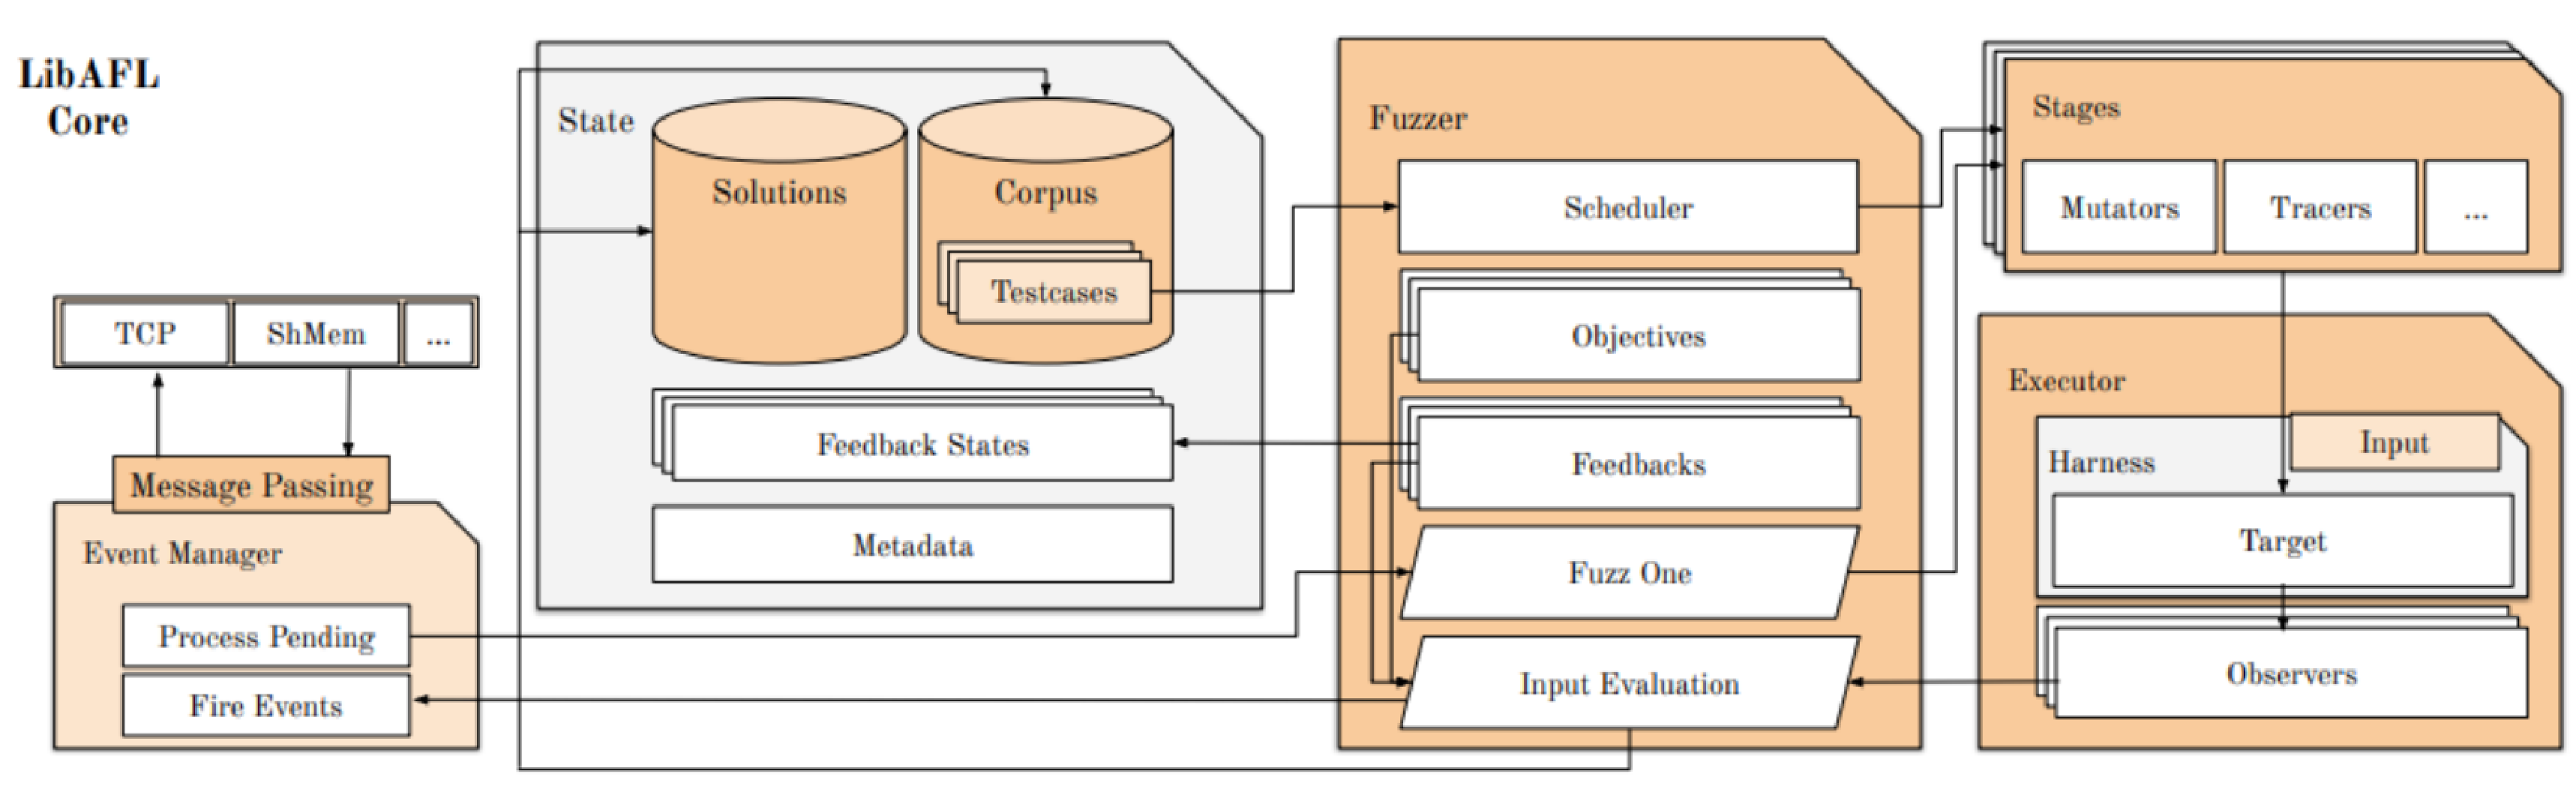
\includegraphics[width=\linewidth]{img/fuzzing/fuzzercore}
\end{center}

\paragraph{Executor:} Si tratta del componente che \textbf{riceve l'input} da parte del fuzzer vero e proprio \textbf{per poi eseguirlo}. Si possono avere diversi livelli di complessità per un executor, il più semplice (per un binario) è un fork server (fork del processo per poi applicare l'input, la fork evita di dover ricaricare il programma in memoria, il che sarebbe troppo lento). 

Altre tipologie di executor, ad esempio per un kernel, dato che non si può caricare un kernel ex novo ad ogni test, usano VM o Hypervisor (wrapper attorno all'executor vero e proprio).

\paragraph{Input:} Rappresentazione astratta della \textbf{tipologia di input accettata} dal programma. Potrebbe essere una bytestring (binario), una sequenza di syscall (kernel), una lista di transazioni (smart contract), \dots; a seconda di ciò che viene testato è importante conoscere cosa prende in input il programma.

\paragraph{Corpus:} Gli input vanno salvati da qualche parte. Il Corpus contiene due elementi:
\begin{itemize}
	\item \textbf{Solutions}: input che assolvono al loro compito; ovvero causano crash o comunque raggiungono l'obiettivo

	\item \textbf{Interesting}: input che raggiungono zone \textit{interessanti} del programma (e quindi vengono messi in coda per eventuale mutazione)
\end{itemize}
Quelle non interessanti vengono scartate (a cosa servono?).

\paragraph{Generator:} Il componente che si occupa di generare input, secondo grammatiche o regole di generazione. In generale, gli input generati devono rispettare una struttura.

\paragraph{Scheduler:} Si può avere un numero indefinito di test case (tra generazione e mutazione gli input possono aumentare molto in fretta), quindi è importante orchestrare in maniera corretta la \textbf{selezione dei test case}. Va definito uno scheduler, nel caso più semplice può essere una coda/stack, ma può avere un impatto significativo sulle performance.

\paragraph{Stage:} Definisce una serie di operazioni da effettuare sull'input (ricevuto dallo scheduler), come mutazioni, taint tracking, \dots.

\paragraph{Mutator:} Si occupa della \textbf{mutazione degli input}. A seconda del test case e di ciò che si vuole ottenere ne esistono di diverso tipo, il metodo più semplice è un bit flip, ma anche splicing, block swapping, truncating, \dots; possono essere usate tecniche arbitrariamente complesse.

\paragraph{Observer:} Si vuole avere conoscenza di ciò che accade all'interno del programma, al fine di definire \textit{cosa è interessante} (tranne nei casi di fuzzer black box, dove non si ha la nozione di interessante, vanno più o meno a caso, le uniche cose interessanti sono le soluzioni). 

L'observer si occupa di \textbf{estrarre} (in qualche modo) \textbf{informazioni dal programma} in fase di analisi per poi rimandarle al fuzzer. 

Un esempio potrebbe essere una coverage map: controlla gli edge, vengono tracciati i possibili flussi di esecuzione e si tiene traccia in un bytearray di quante volte l'esecuzione passa attraverso ogni determinata zona del programma.

\paragraph{Feedback:} Modulo che si occupa di \textbf{analizzare le informazioni estratte}, controparte dell'observer. Riceve l'output dell'observer, lo analizza per determinare caratteristiche riguardo al test case eseguito, ad esempio per stabilire se è interessante e aggiungerlo o meno al corpus.

Cosa manca? Altri componenti che potrebbero esserci, meno nel dettaglio: 
\begin{itemize}
    \item se il fuzzer è su una macchina diversa dall'eseguibile, bisogna collegarlo alla rete
    \item \textbf{Harness}: sotto-componente dell'executor che effettivamente passa l'input al programma
\end{itemize}

\subsubsection{Instrumentation}

\textit{Come si fa a implementare un observer?} Vogliamo estrarre informazioni da un programma a runtime, solitamente si fa con tecniche di \textbf{instrumentazione}: tipicamente a partire da una intermediate representation (per poterlo analizzare più facilmente in maniera automatica, senza rischiare di modificare il comportamento originario del programma), si analizza il programma per identificare zone "interessanti" e si aggiungono istruzioni che permettono di capire quando queste vengono raggiunte. 

Esempio: mi interessa (per qualche motivo) contare le chiamate di sistema del programma, cerco all'interno della intermediate representation tutte le istanze di syscall e assegno un ID ad ognuna di queste, il codice iniettato tramite instrumentazione incrementerà in un array la casella corrispondente alla syscall effettuata, per ogni chiamata all'interno del programma. 

Altro esempio di instrumentazione: i fat pointer, obiettivo diverso, ma sostanzialmente è la stessa cosa (visti qui: \ref{par:fat-pointers}). 

\paragraph{TL;DR:} Instrumentazione vuol dire modificare il binario (solitamente non da sorgente, ma da rappresentazione intermedia), per rilasciare informazioni a runtime.

\subsubsection{Sanitizers}

Vogliamo identificare crash del programma, ma potrebbe non bastare per trovare vulnerabilità. Per questo motivo sono nati i sanitizer, pezzi di codice, \textbf{instrumentazioni aggiuntive} che permettono di \textbf{rilevare comportamenti anomali} quando accadono. 

Esempi: 
\begin{itemize}
	\item \href{https://github.com/google/sanitizers/wiki/addresssanitizer}{\texttt{AddressSanitizer (ASan)}}, rileva errori di memoria

	\item \href{https://docs.kernel.org/dev-tools/ubsan.html}{\texttt{UndefinedBehaviorSanitizer (UBSan)}}, rileva undefined behavior

	\item \href{https://github.com/google/sanitizers/wiki/threadsanitizercppmanual}{\texttt{ThreadSanitizer (TSan)}}, rileva race conditions
\end{itemize}

Quando rilevano un'anomalia fanno crashare il programma, con un log relativo all'errore, il quale può essere più o meno dettagliato.

Esempio: ASan (tra le altre cose) aggiunge delle "red zone" attorno alle zone di memoria, ovvero zone senza permessi di lettura o scrittura: quando il programma prova ad accedervi si genera un \texttt{segfault}. Instrumenta il programma per cercare tutte le allocazioni, tutti gli utilizzi della memoria in generale (con le relative ottimizzazioni, non così semplice).

Ovviamente i sanitizer non vengono usati in produzione, non si tratta di un comportamento desiderato, oltre al fatto che rallentano l'esecuzione.

\vfill

\subsection*{Notes}

\paragraph{State of the Art: AFL++:} Stato dell'arte per fuzzing su binario, \href{https://www.usenix.org/system/files/woot20-paper-fioraldi.pdf}{\texttt{presentato nel 2020}} come gray box fuzzer con edge coverage guidance, derivato dall'originale AFL. Abbastanza customizzabile, scritto in C++. 

\paragraph{NB:} Si può fuzzare un po' tutto, non solo binari. Ad esempio:
\begin{itemize}
	\item \href{https://github.com/google/syzkaller}{\texttt{Syzkaller:}} unsupervised coverage-guided kernel fuzzer

	\item \href{https://softsec.kaist.ac.kr/~sangkilc/papers/choi-ase2021.pdf}{\texttt{Smartian:}} Smart Contract Fuzzing with static and dynamic data-flow analyses

	\item \href{https://dl.acm.org/doi/pdf/10.1145/3492321.3519591}{\texttt{Nyx-Net:}} coverage-guided network testing
\end{itemize}

\paragraph{OSS-Fuzz:} Progetto lanciato da Google nel 2016 per fare fuzzing di repo open source di grossi progetti, individuando un buon numero di vulnerabilità in più di 1000 progetti.

% End L10